\documentclass{beamer}
\usepackage[utf8]{inputenc}
\usepackage[T1]{fontenc}
\usepackage[english]{babel}
\usepackage{amssymb}
\usepackage{soul}
\usepackage{listings}
\usepackage{alltt}
\usepackage{underscore}
\usepackage{verbatim}
\usepackage{graphicx}
\usepackage{ae}
\usepackage{amsmath}
\usepackage{amsfonts}
\PassOptionsToPackage{pdflatex}{graphicx}
\usepackage{pgfpages}
\usepackage{algorithm}


\usepackage{tabularx}
\usepackage{placeins}
\usepackage[noend]{algpseudocode}
\usepackage{caption}
\usepackage{subcaption}

\usepackage{graphicx,eso-pic}

\algdef{SE}[DOWHILE]{Do}{doWhile}{\algorithmicdo}[1]{\algorithmicwhile\ #1}%
\newcommand{\abs}[1]{\lvert#1\rvert}
\newcommand{\norm}[1]{\lVert#1\rVert}


\usetheme{Warsaw}
\graphicspath{ {images/} }

\definecolor{listinggray}{gray}{0.9}
\definecolor{lbcolor}{rgb}{0.9,0.9,0.9}


\setbeameroption{show notes}
\setbeameroption{show notes on second screen=right}

\usefonttheme{professionalfonts}


\title[Degree Project]{Degree Project}
\subtitle{Extending IIQS to support sequences with repeated elements} 
\author[E. Regla]{Erik Regla} 
\institute[UTalca]{Universidad de Talca}
\date{\today} 

\begin{document}

\begin{frame}
  \titlepage
\end{frame}


\begin{frame}{Overview}
    \tableofcontents
    \note{La estructura de esta presentación se divide en los siguientes puntos:}
\end{frame}

\section{Introduction}
\subsection{Context}
\begin{frame}{Introduction}
    \note{La estructura de esta presentación se divide en los siguientes puntos:}
\end{frame}


\subsection{Goals}
\begin{frame}{Primary Goal}
    \emph{To use an experimental algorithmics approach to design an extension of Introspective Incremental Quick Select which is tolerant to repeated elements in the input sequence}.
    \note[item]{La meta principal de este trabajo es utilizar una metodología de algorimos experimentales para diseñar una extensión de Introspective Incremental Quick Select, el cual sea tolerante a entradas con elementos repetidos.}
    \note[item]{Para lograr estos objetivos, necesitamos previamente completar las siguientes tareas [next_slide]}
\end{frame}

\begin{frame}{Specific Goals}
    \begin{itemize}
        \item Research the foundations of Incremental Quick Select and Introspective Incremental Quick Select.
        \item Plan a series of pilot experiments to gain insight on potential improvements.
        \item Apply this insight to design a new version of our target algorithm.
        \item Empirically prove its correctness by benchmarking it. 
    \end{itemize}

    \note[item]{Investigar respecto a los fundamentos teóricos de Incremental Quick Select y de Introspective Incremental Quick Select, de modo de poder comprender como este funciona y cómo diseñar correctamente una implementación para sus pruebas.}
    \note[item]{Planificar una serie de experimentos piloto los cuales nos permitan obtener información al respecto.}
    \note[item]{Utilizar esta información para diseñar una nueva versión del algoritmo.}
    \note[item]{Finalmente, probar su correctitud de manera empírica por medio de experimentos.}
\end{frame}

\subsection{Methodology}

\begin{frame}{Methodology overview}
    We use \emph{A guide to experimental algorithmics} as our base resource to craft a custom methodology for our problem.
    \note[item]{A modo poder afrontar nuestro desafío de ingeniería de algoritmos, se decidió construir una metodología propia en base a diseño de experimentos.}
    \note[item]{Para estos efectos, se utiliza el libro de Catherine McGeoch \emph{A guide to experimental algorithmics} como guia para el diseño de nuestro proceso.}
\end{frame}

\begin{frame}{Experimental algorithmics}
    \begin{figure}
        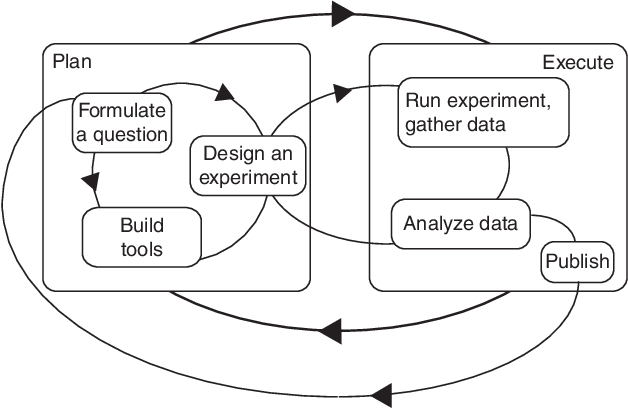
\includegraphics[height=.6\textheight]{eacycle.png}\\
        \caption{Experimental algorithmics cycle}
    \end{figure}
    \note[item]{La extrapolación de la metodología de \emph{Diseño de experimentos} a la ingeniería de algoritmos propuesta por McGeoch presenta el desarrollo de esta como un proceso iterativo compuesto de dos componentes principales.}
\end{frame}

\begin{frame}{Experimental algorithmics}
    \begin{figure}
        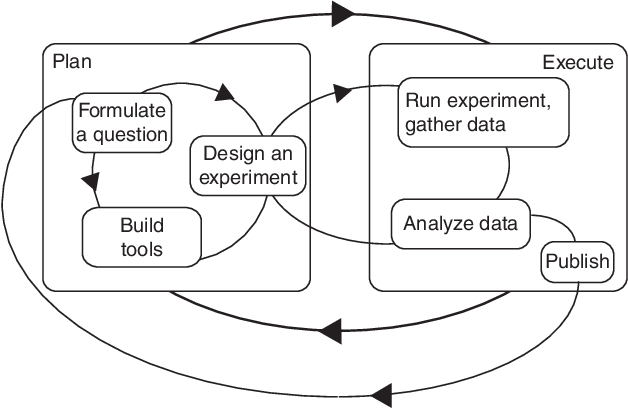
\includegraphics[height=.6\textheight]{eacycle.png}\\
        \caption{Experimental algorithmics cycle}
    \end{figure}
    \note[item]{Por un lado, tenemos la etapa de planificación de nuestros experimentos en las cuales formulamos preguntas y en paralelo diseñamos nuestros experimentos y desarrollamos nuestras herramientas para el estudio.}
\end{frame}

\begin{frame}{Experimental algorithmics}
    \begin{figure}
        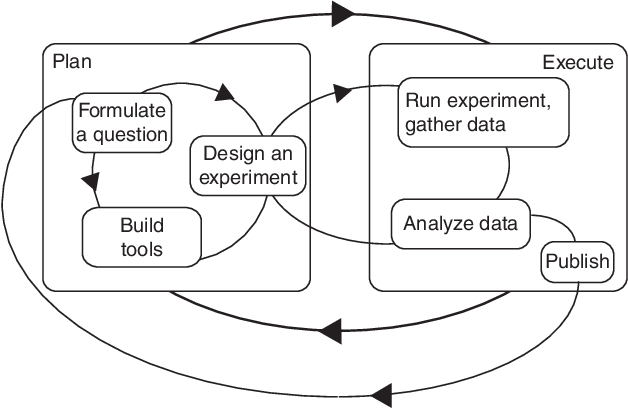
\includegraphics[height=.6\textheight]{eacycle.png}\\
        \caption{Experimental algorithmics cycle}
    \end{figure}
    \note[item]{Por el otro tenemos la ejecución propiamente tal de nuestros experimentos, junto con el análisis e interpretación de nuestros resultados.}
    \note[item]{Hay que destacar que en esta extrapolación tanto las etapas de planificación como ejecución se ejecutan de manera cíclica sin tener un límite definido en las iteraciones ni orden.}
    \note[item]{Esto es asi ya que la etapa de ejecución puede llevarnos a nuevas preguntas y durante la planificación pueden surgir nuevas propuestas. Es tarea de quien ejecuta esta metodología el controlar el proceso.}
\end{frame}

\section{Methodology foundations}
%\note[item]{Nuestra meta es determinar .}

\begin{frame}{Methodology foundations}

    \emph{TODODO}.

    \note[item]{El primer paso en el diseño de nuestra metodología de trabajo es separar las jerarquías de instanciación de algoritmos contra las jerarquías de diseño de algoritmos.}

    \note[item]{Seguido de esto, necesitamos formalizar las etapas de nuestros ciclos. Esto considera el cómo vamos a ejecutar nuestros experimentos, la información que recolectaremos y las consideraciones de iteración.}

    \note[item]{Todo esto está articulado gracias a la investigación previa realizada, sin embargo, cada iteración del proceso afecta el alcance de manera incremental.}

\end{frame}

\subsection{Algorithm instantiation hierarchy}

\begin{frame}{Algorithm instantiation hierarchy}

    \note[item]{Para las jerarquías de instanciación de algoritmos (son los distintos niveles de abstracción de nuestro algoritmo las cuales son específicas de su representación final)...}

    \note[item]{Sabemos de antemano que el paradigma sobre el cual opera IQS e IIQS pertenecen a la familia de algoritmos de ordenamiento interno-adaptivo, basado en particiones. El cual será nuestro objetivo a optimizar.}

\end{frame}


\begin{frame}{Algorithms of interest}
    \scalebox{0.5}{
        \begin{minipage}{1\linewidth}
            \begin{algorithm}[H]
                \caption{IncrementalQuickSort}\label{ALG:IQS}
                \begin{algorithmic}[1]
                \Procedure{$iqs$}{$A,S,k$}
                \If{$k \leq S.top()$}
                \State $S.pop()$
                \Return $A[k]$
                \EndIf
                \State $pivot \gets select(k, S.top()-1)$
                \State $pivot' \gets partition(A,pivot,k, S.top()-1)$
                \State $S.push(pivot')$
                \State \Return $iqs(A,S,k)$
                \EndProcedure
                \end{algorithmic}
            \end{algorithm}
        \end{minipage}%

        \begin{minipage}{0.1\linewidth}
            \hfill
        \end{minipage}%

        \begin{minipage}{1\linewidth}
            \begin{algorithm}[H]
                \begin{algorithmic}[1]
                  \caption{Introspective IncrementalQuickSort}\label{ALG:IIQS}
                  \Procedure{iiqs}{$A, S, k$}
                  \While{$k < S.top()$}
                    \State $pidx \gets random(k,S.top()-1)$
                    \State $pidx \gets partition(A_{k,S.top()-1}, pidx)$
                    \State $m \gets S.top() - k$
                    \State $\alpha \gets 0.3$
                    \State $r \gets -1$
              
                    \If{$pidx < k + \alpha m$}
                      \State $r \gets pidx$
                      \State $pidx \gets pick(A_{r+1,S.top()-1})$
                      \State $pidx \gets partition(A_{r+1,S.top()-1},pidx)$
                    \ElsIf{$pidx > S.top() - \alpha m$}
                      \State $r \gets pidx$
                      \State $pidx \gets pick(A_{k,pidx})$
                      \State $pidx \gets partition(A_{k,r}, pidx)$
                      \State $r \gets -1$
                    \EndIf
              
                    \State S.push($pidx$)
              
                    \If{$r > -1$}
                      \State S.push($r$)
                    \EndIf  
                  \EndWhile
                  \State S.pop()
                  \State \textbf{return} $A_{k}$\label{IIQS_main_cycle}
                  \EndProcedure
                \end{algorithmic}
              \end{algorithm}           
        \end{minipage}%
        }

    \note[item]{Por la naturaleza de ambos algoritmos, estos comparten una serie de rutinas de uso común. Entre las cuales se cuentan}

    \note[item]{Next, encargado de extraer el siguiente elemento (mínimo) en la secuencia -este es el algoritmo en si.}
    \note[item]{Partition, encargado de dividir el arreglo.}
    \note[item]{Swap, encargado de intercambiar elementos.}
    \note[item]{Push y pull, los cuales son operaciones propias de la pila subbyacente.}

    \note[item]{Adicionalmente, tenemos BFPRT y Median que son rutinas de uso exclusivo de IIQS, las cuales son utilizadas de acuerdo al resultado de la evaluación de salud de la ejecución.}

\end{frame}

\begin{frame}{Implementation and execution concerns}

    \note[item]{Nuestro programa fuente para la ejecución de los experimentos será C++ en conjunto de Boost para apoyar el paso de argumentos al binario resultante.}

    \note[item]{Respecto al código objeto, este es obtenido por compilación directa de nuestro código fuente, automatizado por medio de Makefiles sin tratamiento especial de los artefactos resultantes.}
    \note[item]{A nivel de proceso, todos nuestros experimentos son ejecutados sobre espacio de usuario sin privilegios adicionales de ejecución.}

\end{frame}


\subsection{Algorithm design hierarchy}

\begin{frame}{Algorithm design hierarchy}

    \note[item]{Ahora, las jerarquías de diseño de algoritmos (que son la separación lineal de su implementación desde su representación abstracta hasta su implementación)...}

    \note[item]{Tenemos que nuestros sujetos a experimentación estan diseñados de manera de prioritizar la flexibilidad de ejecucucion por sobre la convención.}

\end{frame}


\begin{frame}{Design overview}

    \note[item]{Para esto, los binarios a utilizar durante el proceso de experimentación fueron diseñados en base a tres unidades principales.}

    \note[item]{El ejecutor principal, quien es el encargado de recibir los argumentos de nuestro programa, configurar y ejecutar los experimentos sobre nuestros algoritmos.}

    \note[item]{La especificación de snapshots, al cual permite la recolección y almacenaje de datos de manera estructurada. }

    \note[item]{Los cronómetros que ejecutan las detenciones del código para perfilar su ejecución, los cuales están implementados utilizando el sistema de macros provisto por C para ejecutar los cambios en la etapa de precompilacion.}

\end{frame}


\begin{frame}{Implementation overview}

    \note[item]{A modo de mejorar la replicabilidad de los experimentos se optò por utilizar un sistema de aleatorización sistemática combinado con un inicialización fija de parámetros iniciales. De esta manera nuestra ejecucucion cuenta con una única fuente de verdad.}

    \note[item]{Por otro lado para poder mejorar la calidad de los resultados, se optó por declarar globalmente una instancia única de snapshots junto con pre-alocación de memoria de manera adelantada para evitar interferencias de llamadas a sistema para tales efectos.}

\end{frame}
    

\subsection{Experimental process breakdown}


\begin{frame}{Metrics}

    \note[item]{Dentro de las métricas definidas para nuestro proceso de experimentación contamos:}

    \note[item]{Número de intercambios, el cual tiene propósitos de verificación.}
    \note[item]{Operaciones de la pila, la cual ya en los trabajos previos se ha visto que estas se manifiestan de forma directa en el tamaño que esta tiene a lo largo de cada extracción e impacta directamente en el tiempo de ejecución.}
    \note[item]{Y el tiempo de ejecución.}

\end{frame}
    


\section{Pilot experiments}

\subsection{Partitioning algorithms}

\begin{frame}{Partitioning repeated elements}

    \note[item]{Antes de comenzar con los experimentos necesitamos asegurarnos que nuestra implementación de IQS no caiga en casos donde este no pueda responder.}
    \note[item]{Ya que la implementación no especifica el mecanismo de particionado, cambiamos nuestra versión de el algoritmo de particionado a una versión compatible con secuencias repetidas.}

\end{frame}




\subsection{Base benchmarks}

\begin{frame}{Base benchmark}
    \begin{figure}
        \centering
        \begin{subfigure}[b]{\textwidth}
            \centering
            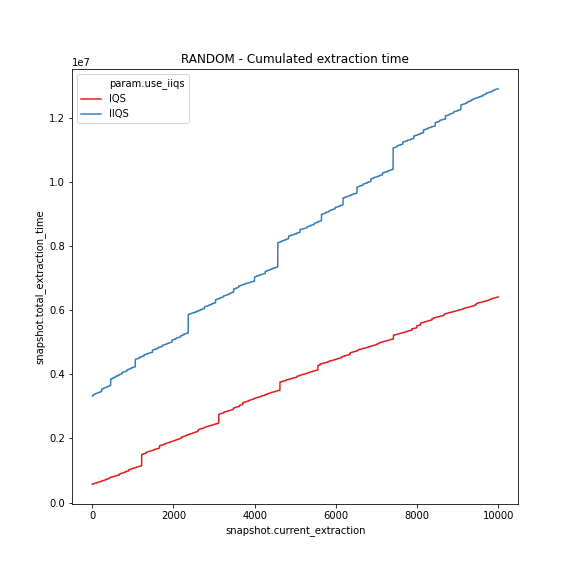
\includegraphics[height=0.42\textheight]{chapter4/01-basebenchmark-01-random-case.png.0-0.png}
            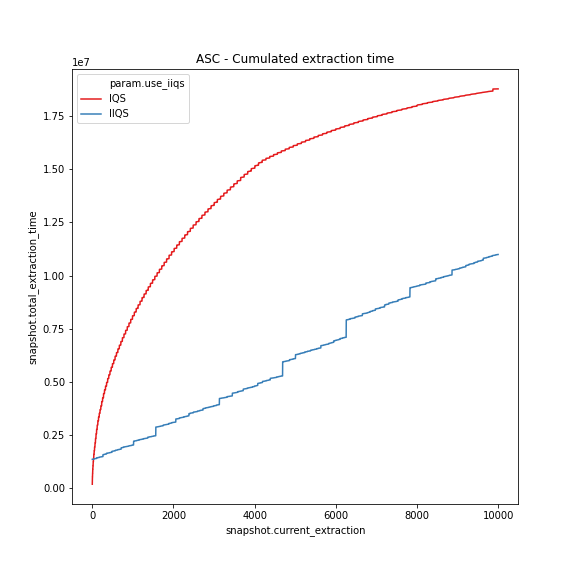
\includegraphics[height=0.42\textheight]{chapter4/01-basebenchmark-02-sort-a-case.png.0-0.png}
            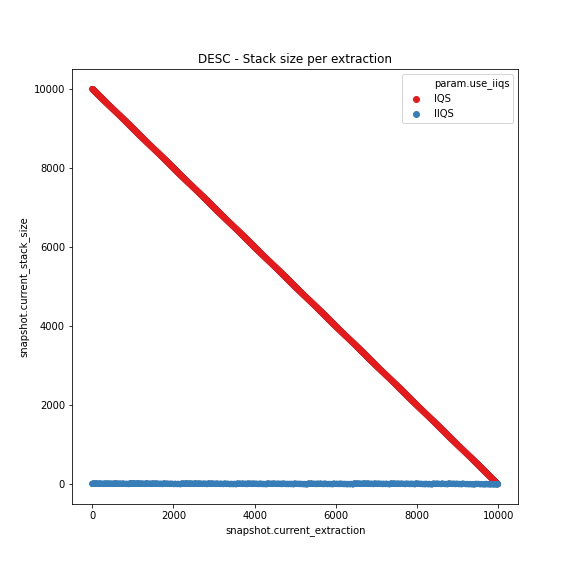
\includegraphics[height=0.42\textheight]{chapter4/01-basebenchmark-03-sort-d-case.png.2-0.png}
        \end{subfigure}
        \caption{Base IQS and IIQS benchmark.}
    \end{figure}
    \note[item]{Podemos observar que ambos algoritmos se comportan de manera similar cuando la entrada es una secuencia ordenada de manera aleatoria.}
    \note[item]{No a su vez cuando los distintos tipos de entrada cambian a secuencias ordenadas. El preordenamiento de estas secuencias afecta de manera negativa la ejecución de IQS.}
    \note[item]{Si bien el fundamento de ambos algoritmos es exactamente el mismo, la implementación de una evaluacion para el cambio de estrategia de selección de pivotes permite que IIQS mantenga su complejidad temporal.}

    \note[item]{Antes de comenzar con los experimentos necesitamos asegurarnos que nuestra implementación de IQS no caiga en casos donde este no pueda responder.}

    \note[item]{Ya que la implementación no especifica el mecanismo de particionado, cambiamos nuestra versión de el algoritmo de particionado a una versión compatible con secuencias repetidas.}
\end{frame}


\begin{frame}{Partitioning repeated elements}

    \scalebox{0.75}{
        \begin{minipage}{0.5\linewidth}
            \begin{algorithm}[H]
                \caption{Hoare's Partition}\label{ALG:HOARE_PARTITION}
                \begin{algorithmic}[1]
                    \Procedure{$hoare$}{$A, p, r$}
                    \State $x \gets A_p$
                    \State $i \gets p-1$
                    \State $j \gets r+1$
                    \While{$true$}
                        \Do 
                            \State $j \gets j - 1$
                        \doWhile{$A_j \leq x$}
                
                        \Do 
                            \State $i \gets i + 1$
                        \doWhile{$A_j \geq x$}
                
                        \If{$i < j$}
                            \State $swap(A_i, A_j)$
                        \Else
                            \State \Return $j$
                        \EndIf
                    \EndWhile
                    \EndProcedure
                \end{algorithmic}
                \end{algorithm}
        \end{minipage}%

        \begin{minipage}{0.1\linewidth}
            \hfill
        \end{minipage}%

        \begin{minipage}{0.7\linewidth}
            \begin{algorithm}[H]
                \caption{Three-way Partition}\label{ALG:DUTCH_FLAG_PARTITION}
                \begin{algorithmic}[1]
                    \Procedure{$threewaypartition$}{$A, p$}
                    \State $k \gets \norm{A}$
                    \State $i \gets 0$
                    \State $j \gets 0$
                    \While{$j < k$}
                        \If{$A_j < p$}
                            \State $swap(A_i, A_j)$
                            \State $i \gets i+1$
                            \State $j \gets j+1$
                        \ElsIf{$A_j > p$}
                            \State $k \gets k-1$
                            \State $swap(A_i, A_k)$
                        \Else
                            \State $j \gets j+1$
                        \EndIf
                    \EndWhile
                    % \State \Return $i,J,k$
                    \EndProcedure
                \end{algorithmic}
                \end{algorithm}                
        \end{minipage}%
        }
        \vfill

        \note[item]{Para poder soportar el ordenamiento de secuencias repetidas, necesitamos cambiar la implementación utilizada durante el trabajo original de IIQS (la implementación de partición de Hoare para secuencias) por la implementación del problema de la bandera danesa (para repetidos).}
        \note[item]{Habiendo hecho eso, la siguiente pregunta es si este cambio afecta el comportamiento de IQS de alguna manera. Ya que teóricamente, para efectos de diseño del algoritmo, si bien su complejidad asintótica permanece de igual manera, la forma en la cual los elementos se mueven dentro del arreglo es diferente.}
\end{frame}



\begin{frame}{Partitioning repeated elements}

    \begin{figure}
        \centering
        \begin{subfigure}[b]{\textwidth}
            \centering
            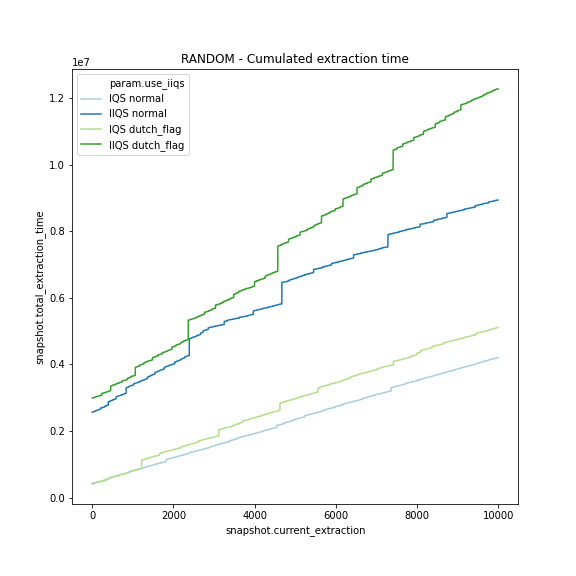
\includegraphics[height=0.4\textheight]{chapter4/02-basebenchmark-01-base-benchmark.png.0-0.png}
            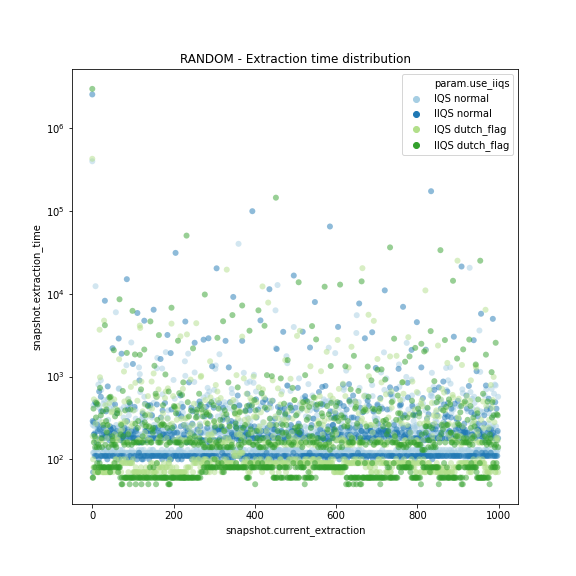
\includegraphics[height=0.4\textheight]{chapter4/02-basebenchmark-01-base-benchmark.png.1-1.png}
            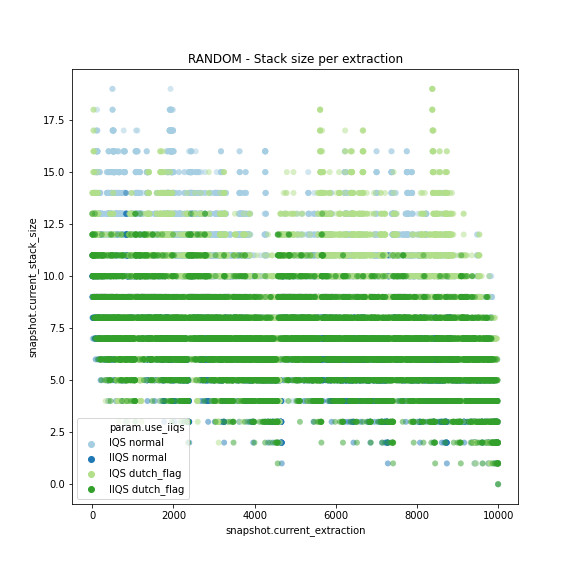
\includegraphics[height=0.4\textheight]{chapter4/02-basebenchmark-01-base-benchmark.png.2-0.png}
        \end{subfigure}
        \caption{Base IQS and IIQS benchmark for a random sequence with $1\times10^5$ elements.}
    \end{figure}

    \note[item]{Podemos observar que la implementación de una estrategia de particionado de tres vías no altera la complejidad para el caso aleatorio, mostrando el mismo comportamiento en ambos algoritmos.}

\end{frame}


\begin{frame}{Ascending sequences}
    \begin{figure}
        \centering
        \begin{subfigure}[b]{\textwidth}
            \centering
            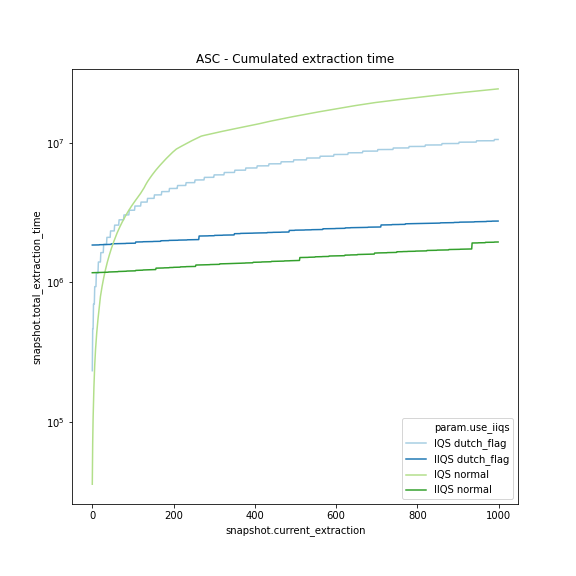
\includegraphics[height=0.4\textheight]{chapter4/02-benchmark-02-sort-a-case.png.0-1.png}
            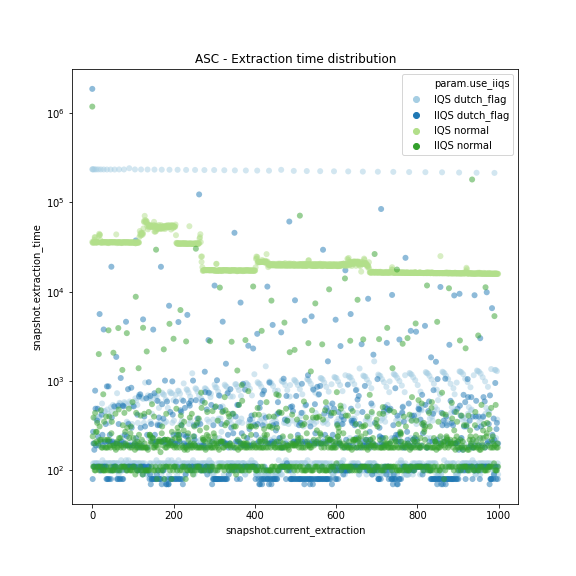
\includegraphics[height=0.4\textheight]{chapter4/02-benchmark-02-sort-a-case.png.1-1.png}
            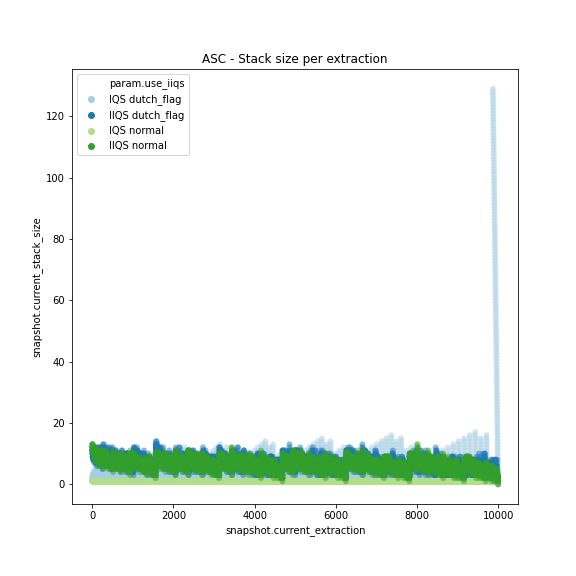
\includegraphics[height=0.4\textheight]{chapter4/02-benchmark-02-sort-a-case.png.2-0.png}
        \end{subfigure}
        \caption{Base IQS and IIQS benchmark for a ascending sequence with $1\times10^5$ elements.}
    \end{figure}
    \note[item]{Podemos apreciar también que para el caso de secuencias ascendentes existe un degrade progresivo de la ejecución dado al pobre uso que se le da a la pila.}
    \note[item]{Esto repercute especialmente al final de la ejecución, debido al ordenamiento hecho por la versión ajustada de nuestro particionador.}
\end{frame}

\begin{frame}{Descending sequences}
    \begin{figure}
        \centering
        \begin{subfigure}[b]{\textwidth}
            \centering
            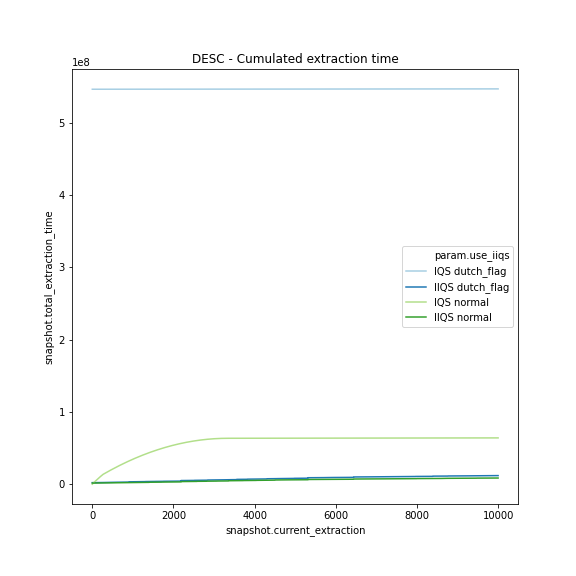
\includegraphics[height=0.4\textheight]{chapter4/02-basebenchmark-03-sort-d-case.png.0-0.png}
            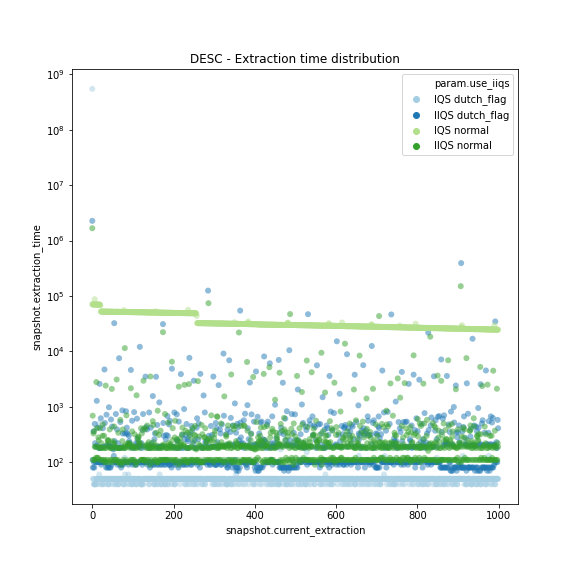
\includegraphics[height=0.4\textheight]{chapter4/02-basebenchmark-03-sort-d-case.png.1-1.png}
            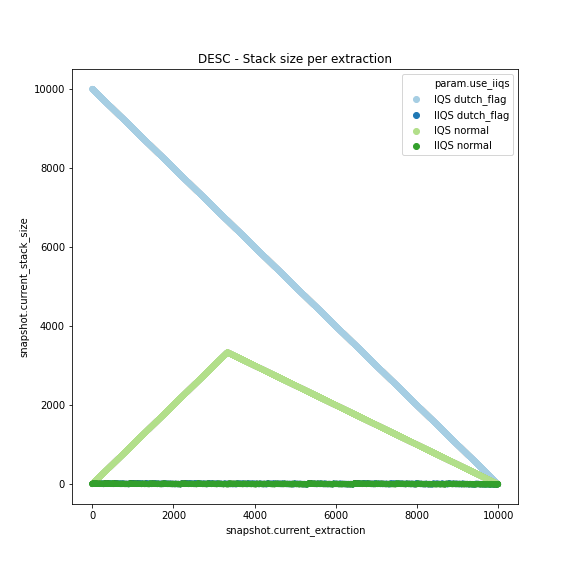
\includegraphics[height=0.4\textheight]{chapter4/02-basebenchmark-03-sort-d-case.png.2-0.png}
        \end{subfigure}
        \caption{Base IQS and IIQS benchmark for a descending sequence with $1\times10^5$ elements.}
    \end{figure}
    \note[item]{Finalmente este fenomeno repercute de manera negativa cuando la secuencia es decreciente, ya que todos los pivotes son almacenados en la pila.}
    \note[item]{A este punto, podemos decir que la implementación del algoritmo de particionado de tres vias, si bien realiza un cambio en el comportamiento de IQS, este sigue manifestando su misma complejidad y falencias.}
\end{frame}

\begin{frame}{Repeating elements}
    \begin{figure}
        \centering
        \begin{subfigure}[b]{\textwidth}
            \centering
            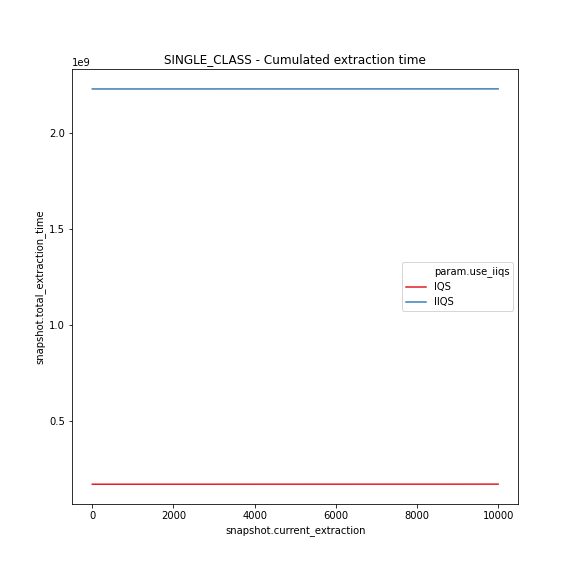
\includegraphics[height=0.4\textheight]{chapter4/01-basebenchmark-04-single-class.png.0-0.png}
            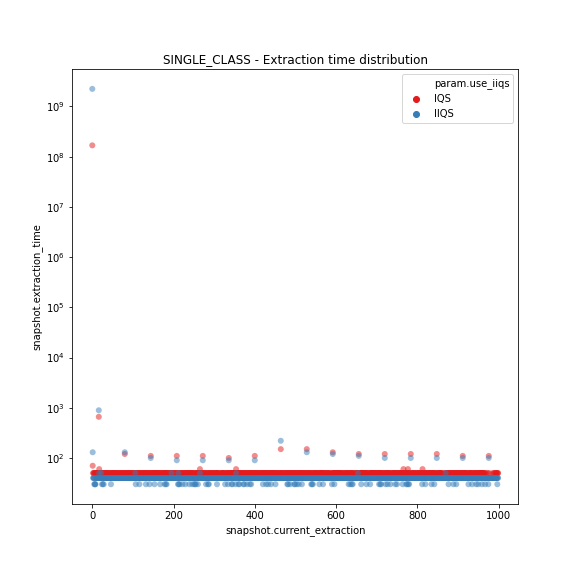
\includegraphics[height=0.4\textheight]{chapter4/01-basebenchmark-04-single-class.png.1-1.png}
            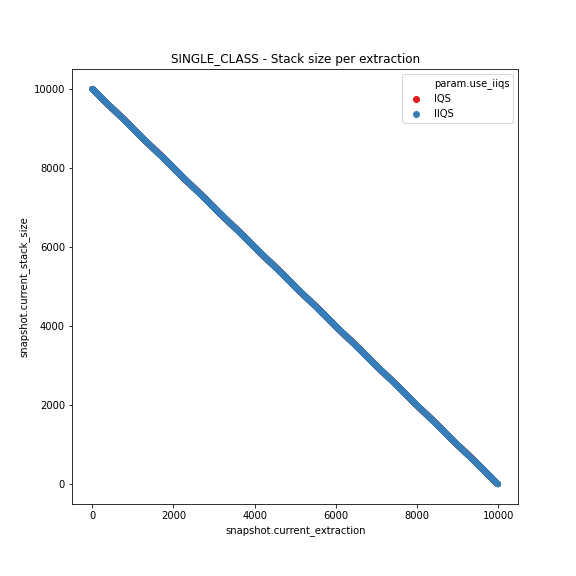
\includegraphics[height=0.4\textheight]{chapter4/01-basebenchmark-04-single-class.png.2-0.png}
        \end{subfigure}
        \caption{Base IQS and IIQS benchmark for a sequence with $1\times10^5$ repeated elements.}
    \end{figure}
    \note[item]{Cuando todos los elementos son iguales, IIQS se comporta igual que IQS en su peor caso.}
\end{frame}


\begin{frame}{Class impact}
    \begin{figure}
        \centering
        \begin{subfigure}[b]{\textwidth}
            \centering
            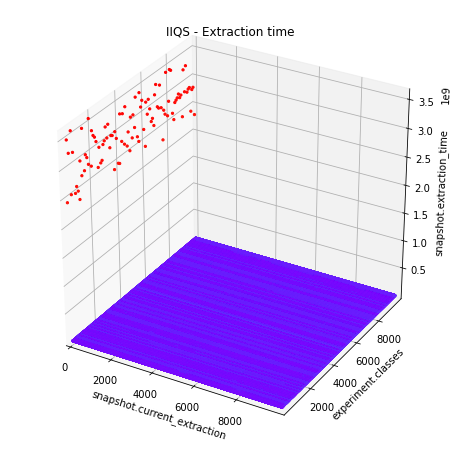
\includegraphics[height=0.6\textheight]{chapter4/01-basebenchmark-05-classes.png.0-1.png}
            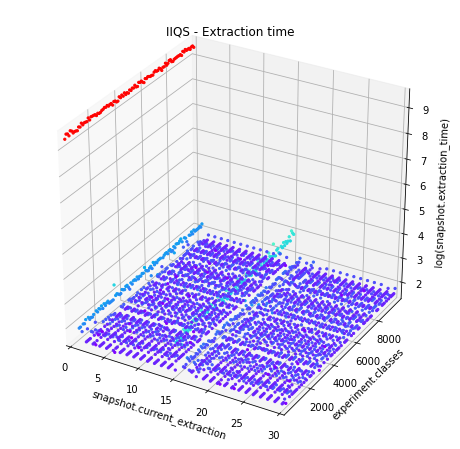
\includegraphics[height=0.6\textheight]{chapter4/01-basebenchmark-05-classes.png.0-2.png}
        \end{subfigure}
        \caption{Impact of classes on IIQS execution.}
    \end{figure}
    \note[item]{Al variar el numero de clases dentro de nuestra secuencia de entrada, nos damos cuenta que existe una diferencia de sobre 8 órdenes de magnitud.}
    \note[item]{Sin embargo, esta solo ocurre cuando hay una clase presente. Esto es porque en el momento que hay una segunda clase, si la clase mayoritaria no cuenta con el 50 porciento de los datos, entonces ese segmento, causante del fenómeno solo representa la mitad de los elementos. En cuyo caso, de pasar por un proceso de particionamiento, ya reduce la complejidad del problema a la mitad.}
    \note[item]{Esta es la primer indicio que si podemos eliminar esa clase mayoritaria o bien controlar la distribución de los elementos, podemos evitar este nuevo peor caso.}
\end{frame}



\begin{frame}{Pivot bias impact}
    \begin{figure}
        \centering
        \begin{subfigure}[b]{\textwidth}
            \centering
            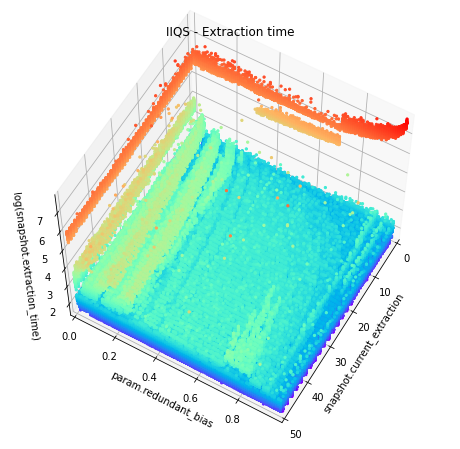
\includegraphics[height=0.6\textheight]{chapter4/01-basebenchmark-07-extraction-bias.png.0-1.png}
            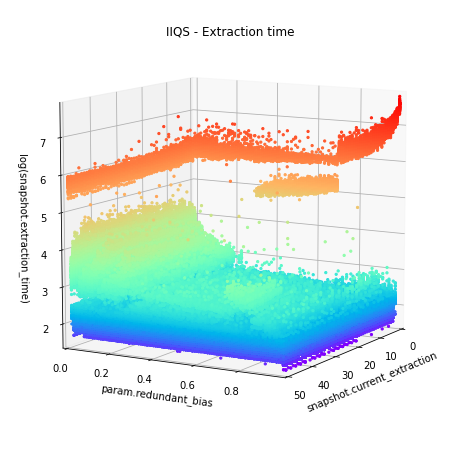
\includegraphics[height=0.6\textheight]{chapter4/01-basebenchmark-07-extraction-bias.png.0-2.png}
        \end{subfigure}
        \caption{Impact of classes on IIQS execution.}
    \end{figure}
    \note[item]{El sesgo de la elección del pivote a devolver durante la etapa de partición de tres vias adolece del mismo problema del peor caso de IQS. Este es, un impacto directo sobre como los elementos son rescatados y de como la pila es usada.}
\end{frame}


\begin{frame}{Random noise impact}
    \begin{figure}
        \centering
        \begin{subfigure}[b]{\textwidth}
            \centering
            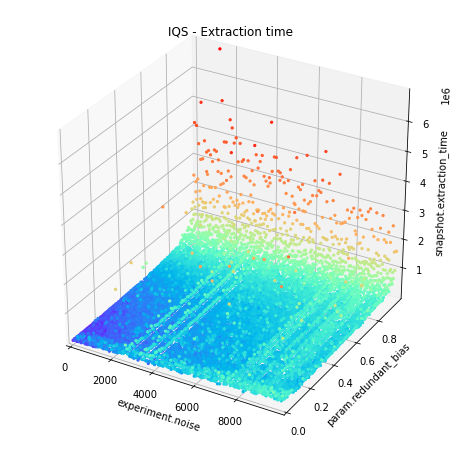
\includegraphics[height=0.6\textheight]{chapter4/01-basebenchmark-06-noise-bias.png.1-0.png}
            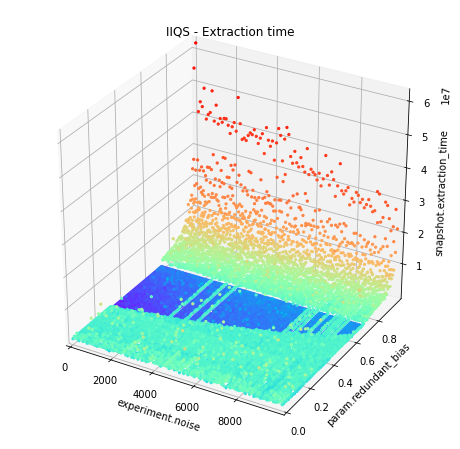
\includegraphics[height=0.6\textheight]{chapter4/01-basebenchmark-06-noise-bias.png.0-0.png}
        \end{subfigure}
        \caption{Impact of classes on IQS and IIQS execution.}
    \end{figure}
    \note[item]{Esta es la primer indicio que si podemos eliminar esa clase mayoritaria o bien controlar la distribución de los elementos, podemos evitar este nuevo peor caso.}
\end{frame}


\begin{frame}{IIQS parameters impact}
    \begin{figure}
        \centering
        \begin{subfigure}[b]{\textwidth}
            \centering
            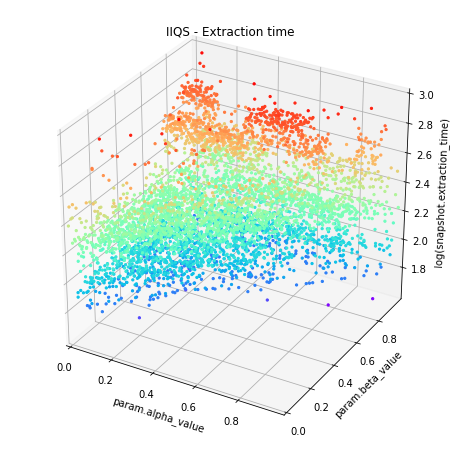
\includegraphics[height=0.38\textheight]{chapter4/04-alphabeta-noclass.png.0-0.png}
            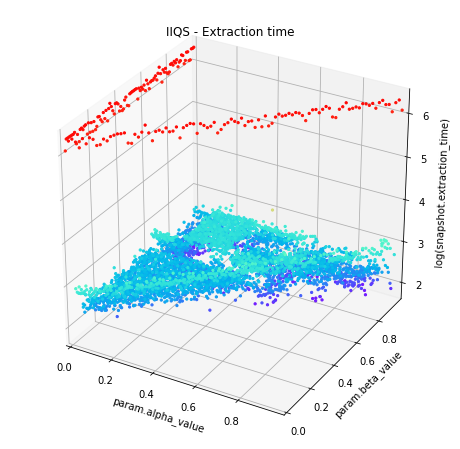
\includegraphics[height=0.38\textheight]{chapter4/04-alphabeta-noclass-asc.png.0-0.png}
            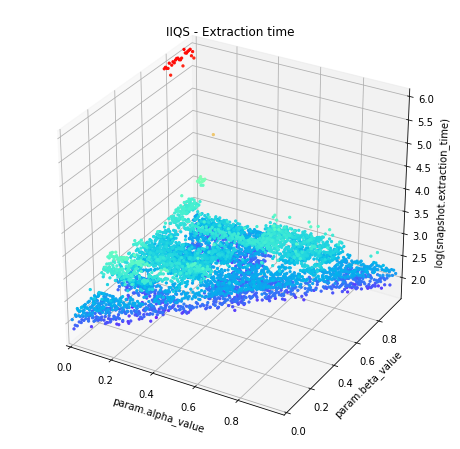
\includegraphics[height=0.38\textheight]{chapter4/04-alphabeta-noclass-desc.png.0-0.png}
            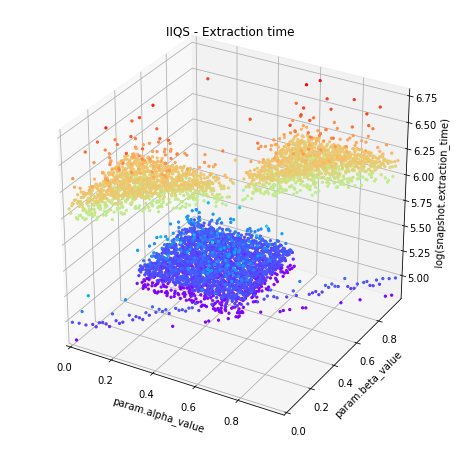
\includegraphics[height=0.38\textheight]{chapter4/04-alpabeta-singleclass.png.1-0.png}
        \end{subfigure}
        \caption{Impact of $\alpha$ and $\beta$ on IIQS for unique sequences.}
    \end{figure}

    \note[item]{Por otro lado, no vemos relación alguna entre los comportamientos esperados para el caso de secuencias con elementos únicos a con una única secuencia. Es mas, incluso el mejor tiempo de ejecucucion es comparable a los peores casos vistos de elección de los parámetros alpha y beta.}
    \note[item]{Esto nos advierte inmediatamente que la posibilidad de poder ejecutar mejoras a nivel de los parámetros de IIQS no existe ya que no tiene mayor papel.}
    \note[item]{Entonces, sabemos que el problema de este caso es el número de clases.}
    \note[item]{Sabemos también que si logramos hacer que la clase mayoritaria ocupe menos del 50 porciento, volvemos a un caso esperado de ejecución.}
    \note[item]{Sabemos también que si logramos hacer que la clase mayoritaria ocupe menos del 50 porciento, volvemos a un caso esperado de ejecución.}
\end{frame}

\section{Workhorse experiment}

\begin{frame}{Idea pt. 1}
    Our sorting problem does not take into account the position of the elements and only relies on the value of such elements. This allows us to use the mapping induced by counting sort, $C_{in}$, as a intermediate representation of our original sequence $S_{in}$.

    \note[item]{Sabemos que la familia de algoritmos derivados directamente de iqs son algoritmos de ordenamiento adaptivo. Esto quiere decir que su tiempo de ejecución va en función de la entrada.}
    \note[item]{Entonces, la idea principal es convertir directamente la entrada por medio de un proceso auxiliar, de modo que sea compatible con IQS/IIQS.}
\end{frame}
    

\begin{frame}{Idea pt. 2}
    Let us define $S_{repeated(\gamma)}$ as a sequence $(s_0, s_1,...,s_{n-1},s_{n})$ on which $\forall ~s_i \in [0,n]:~s_i = \gamma$. Then every sequence $S_in$ can be seen as a concatenation of $m$ sequences of size $k$ on which $k \leq m$. Then we can establish two functions $roll$ and $unroll$ defined as follows:
    \begin{align*}
        roll \colon S_{repeated(\gamma)} &\to C_{\gamma}\\
        (s_0, s_1,...,s_{n-1},s_{n})  &\mapsto (n).
    \end{align*}
    
    And analogously:
    \begin{align*}
        unroll \colon C_{\gamma} &\to S_{repeated(\gamma)}\\
        (n) &\mapsto (s_0, s_1,...,s_{n-1},s_{n}).
    \end{align*}

    \note[item]{Estas dos funciones roll y unroll que modelan funcionan a nivel de elemento.}
    \note[item]{Por tanto podemos extender su definición a secuencias ordenadas concatenando estos elementos S sub gamma.}
\end{frame}


\begin{frame}{Integration strategies}
    This mapping allows us to represent any sequence of elements as a sequence of pairs which represent the element and how many repetitions of this element are concatenated to it.\footnote{This representation is also known as \emph{frequency table}.}\\
    \vfill

    As both $roll$ and $unroll$ functions operate per each element and not at sequence level we can extend their usage both inside of our current IQS and IIQS implementation or as a external process.\\

    \note[item]{Lo que estamos haciendo, es definir de manera modular la implementación de un ordenamiento por conteo o una tabla de frecuencias.}
    \note[item]{Esto nos permite agregar esta reducción como un proceso externo o interno a nuestro algoritmo objetivo}
\end{frame}


\begin{frame}{High-level external implementation}

    We denote our candidate sorting algorithm as an anonymous function $\lambda_{sort}$. Then our external reduction strategy is as follows:
    \vfill
    \scalebox{0.75}{
        \begin{minipage}{1\linewidth}
            \begin{algorithm}[H]
            \caption{External reduction}\label{ALG:EXTERNAL_IQS}
            \begin{algorithmic}[1]
                \Procedure{$external\_strategy$}{$S_{in}, k, \lambda_{sort}$}
                \State $C_{in} \gets roll(S_{in})$
                \State $S_{sorted}' \gets \lambda_{sort}(C_{in}, S, k)$
                \State $S_{out}' \gets [~]$
                \For{$s \in S_{sorted}'$}
                    \State $S_{out}' \gets S_{out}'~^\frown~unroll(s, C_{in}(s))$
                \EndFor
                \State \Return $S_{out}$
                \EndProcedure
            \end{algorithmic}
            \end{algorithm}
        \end{minipage}%
    }
    \vfill
    As both $roll$ and $unroll$ functions operate per each element and not at sequence level we can extend their usage both inside of our current IQS and IIQS implementation or as a external process.\\

    \note[item]{Nuestra estrategia se reduce entonces a ejecutar una reducción de la entrada mapeandola a un conjunto de pares (llave, valor), ordenar las llaves y posteriormente al momento de retornar los elementos, consumir estos por medio de nuestra función de mapeo.}

\end{frame}
    


\begin{frame}{High-level external implementation}
    We asume that roll operation as it is an instance of counting sort it takes $O(n)$ time and line 4 onwards also take $O(n)$.  \vfill

    As the average running time for IQS and IIQS is $O(n~+~k~log_2(k))$, then the addition of our external strategy to deal with repeating elements introduces a fixed $n + l$ overhead on which $l$ denotes the number of classes present on $S_{in}$. \vfill
    
    In worst case, $l~=~\norm{S_{in}}$, which is suboptimal in relation to IQS.

    \note[item]{Este overhead introducido por el proceso externo, si bien mantiene la complejidad temporal, no conserva la complejidad espacial, ya que en peor caso, necesitamos $n$ extra espacio para poder ejecutar el ordenamiento debido a una tabla de frecuencias con puros unos.}

    \note[item]{Resulta obvio que no es posible aplicar esta estrategia a IQS ya que no tenemos manera de controlar la distribución de las llaves de los retornados por la tabla de frecuencia. De modo que esta implementación no es factible. }
\end{frame}



\begin{frame}{High-level internal implementation}

    By extending the operations involved IIQS, the stack store pairs of elements $u = (p_{start}, p_{end})$ on which $p_{start}$ is the first position of the pivot and $p_{end}$ is the frequency on the array.

    \vfill
    \scalebox{0.75}{
        \begin{minipage}{.6\linewidth}
        
            \begin{algorithm}[H]
                \caption{Binned Stack top}\label{ALG:STACK_TOP}
                \begin{algorithmic}[1]
                    \Procedure{$Stack.binnedTop$}{$S$}
                    \State $(p_{start}, p_{end}) \gets S.top()$
                    
                    \State \Return $p_{start}$
                    \EndProcedure
            \end{algorithmic}
            \end{algorithm}

        \end{minipage}%

        \begin{minipage}{.1\linewidth}
            \hfill
        \end{minipage}%

        \begin{minipage}{.6\linewidth}

        
            \begin{algorithm}[H]
                \caption{Binned Stack pop}\label{ALG:STACK_POP}
                \begin{algorithmic}[1]
                    \Procedure{$Stack.binnedTop$}{$S$}
                    \State $(p_{start}, p_{end}) \gets S.top()$
                    \State $S.pop()$
                
                    \If{$p_{start} < p_{end}$}
                        \State $S.push((p_{start}+1, p_{end}))$
                    \EndIf
                    \EndProcedure
            \end{algorithmic}
            \end{algorithm}

        \end{minipage}%
    }

    \note[item]{Lo primero que hay que hacer para implementar esta extensión de manera interna a IIQS, es darle la capacidad a la pila de almacenar rangos en vez de un solo elemento.}
\end{frame}


\begin{frame}{High-level internal implementation}

    \centering
    \scalebox{0.7}{
        \begin{minipage}{.8\linewidth}
            \begin{algorithm}[H]
                \caption{Binned Three-way Partition}\label{ALG:DUTCH_FLAG_PARTITION_RANGED}
                \begin{algorithmic}[1]
                    \Procedure{$binnedPartition$}{$A, p$}
                    \State $k \gets \norm{A}$
                    \State $i \gets 0$
                    \State $j \gets 0$
                    \While{$j < k$}
                        \If{$A_j < p$}
                            \State $swap(A_i, A_j)$
                            \State $i \gets i+1$
                            \State $j \gets j+1$
                        \ElsIf{$A_j > p$}
                            \State $k \gets k-1$
                            \State $swap(A_i, A_k)$
                        \Else
                            \State $j \gets j+1$
                        \EndIf
                    \EndWhile
                    \State \Return $(i,k)$
                    \EndProcedure
                \end{algorithmic}
                \end{algorithm}
        \end{minipage}%
    }

    \note[item]{Posteriormente, nuestro particionador debe soportar el la devolución de rangos de elementos en vez de solamente un elemento. Esto elimina el sesgo de particionado visto anteriormente.}
\end{frame}


\begin{frame}{Binned IIQS}

    \centering
    \scalebox{0.6}{
        \begin{minipage}{1\linewidth}
            \begin{algorithm}[H]
                \begin{algorithmic}[1]
                  \caption{Binned IIQS} \label{ALG:RANGED_IIQS}
                  \Procedure{b-iiqs}{$A, S, k$}
                  \While{$k < S.binnedTop()$}
                      \State $pidx \gets random(k,S.binnedTop()-1)$
                      \State $pidx, range \gets partition(A_{k,S.binnedTop()-1}, pidx)$
                      \State $m \gets S.binnedTop() - k$
                      \State $\alpha \gets 0.3$
                      \State $\beta \gets 0.7$
                      \State $idx_\alpha \gets k + \alpha m$
                      \State $idx_\beta \gets k + \beta m$
                      \State $r \gets -1$
              
                      \If{$pidx > idx_\beta \wedge idx_\alpha < range $}
                          \State $pidx \gets pick(A_{r+1,S.binnedTop()-1})$
                          \State $pidx, range \gets binnedPartition(A_{r+1,S.binnedTop()-1},pidx)$
                      \EndIf
                      \State $S.push((pidx, range)$)
              
                  \EndWhile
                  \State $S.pop()$
                  \State \textbf{return} $A_{k}$\label{IIQS_main_cycle}
                  \EndProcedure
                \end{algorithmic}
              \end{algorithm}
        \end{minipage}%
    }

    \note[item]{De esta manera sin mayores modificaciones al algoritmo original, obtenemos una versión de IIQS que integra la generación de una tabla de frequencias para poder reducir los casos de entrada al caso esperado de la implementación original.}
\end{frame}




\begin{frame}{BIIQS overview}
    
As both Algorithms~\ref{ALG:STACK_TOP} and ~\ref{ALG:STACK_POP} have $O(1)$ worst-case complexity and Algorithm~\ref{ALG:DUTCH_FLAG_PARTITION_RANGED} maintains $O(n)$ complexity on which $n$ dennotes the number of elements in the sequence to partition.
\vfill
Both expected and worst-case time complexity for this \emph{Binned IntrospectiveIncrementalQuickSort} (\emph{bIIQS} from now on) remains $O(n~+~k~log_2(k))$ and our original $O(log_2(k))$ space complexity is maintained as the stack only doubles its size at most.

\note[item]{Esta versión de IIQS preserva el misma orden de complejidad asintótica tanto temporal como espacial que su versión original.}

\end{frame}

\section{Experimental evaluation}


\begin{frame}{Base benchmark}
    \begin{figure}
        \centering
        \begin{subfigure}[b]{\textwidth}
            \centering
            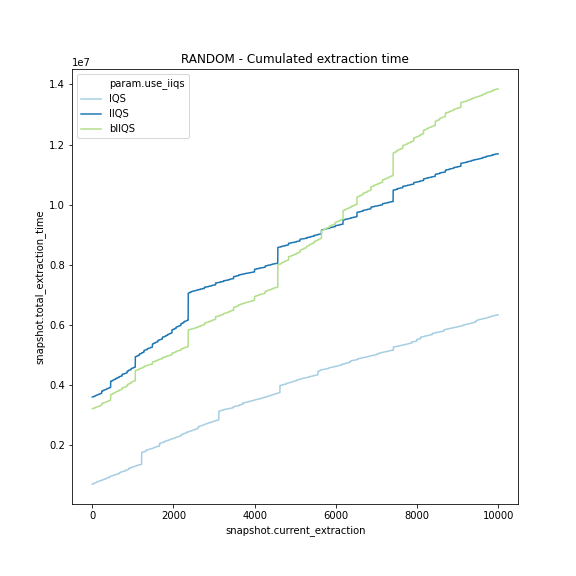
\includegraphics[height=0.45\textheight]{chapter5/01-basebenchmark-01-random-case.png.0-0.png}
            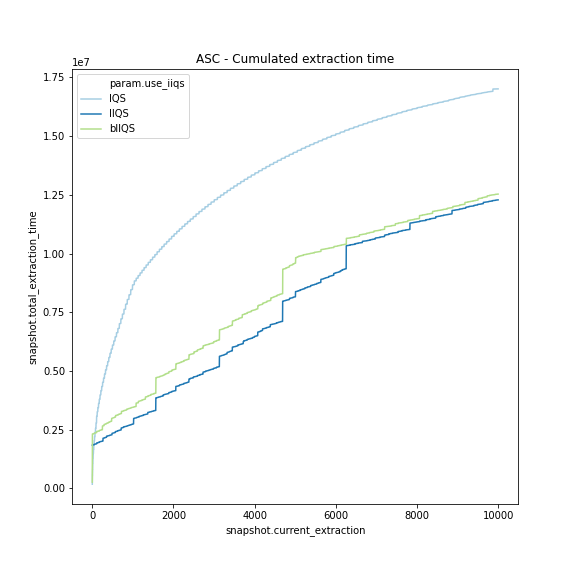
\includegraphics[height=0.45\textheight]{chapter5/01-basebenchmark-02-sort-a-case.png.0-0.png}
            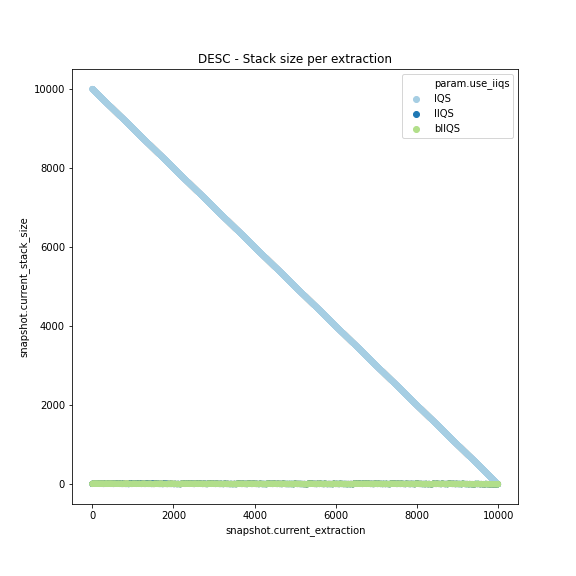
\includegraphics[height=0.45\textheight]{chapter5/01-basebenchmark-03-sort-d-case.png.2-0.png}
        \end{subfigure}
        \caption{BIIQS benchmark.}
    \end{figure}
    \note[item]{Podemos observar que en todas las instancias originales del problema, biiqs entrega los mismos resultados que su versión original.}
\end{frame}


\begin{frame}{Repeating elements}
    \begin{figure}
        \centering
        \begin{subfigure}[b]{\textwidth}
            \centering
            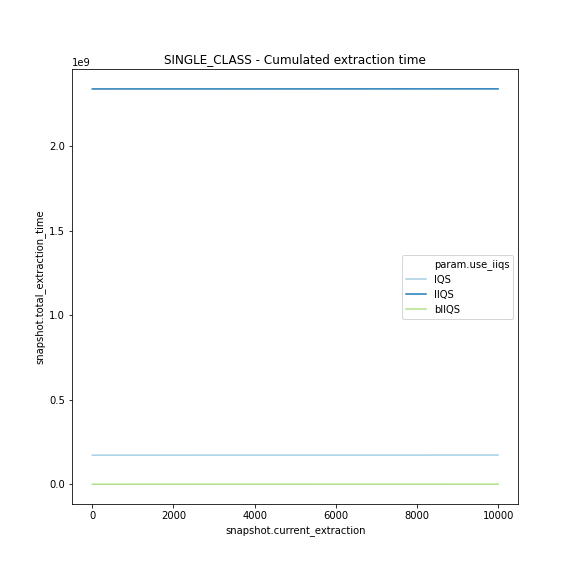
\includegraphics[height=0.4\textheight]{chapter5/01-basebenchmark-04-single-class.png.0-0.png}
            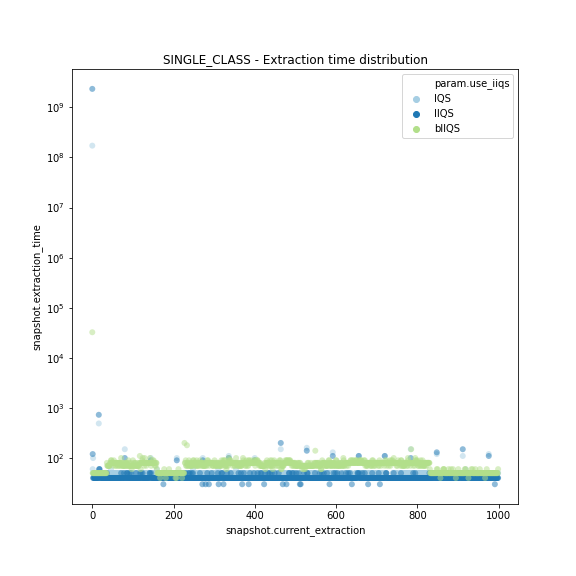
\includegraphics[height=0.4\textheight]{chapter5/01-basebenchmark-04-single-class.png.1-1.png}
            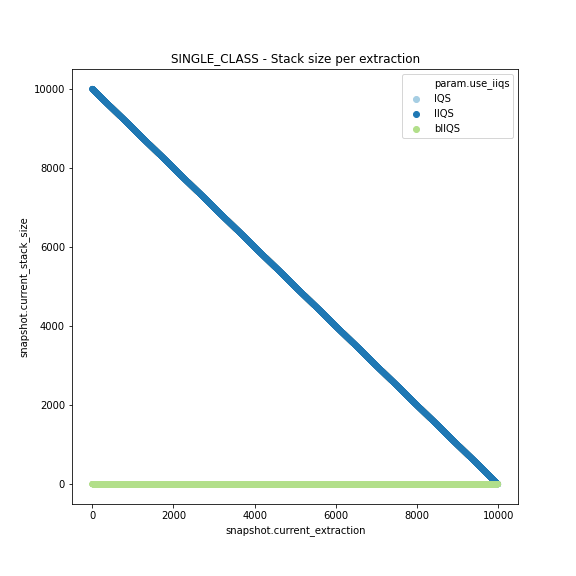
\includegraphics[height=0.4\textheight]{chapter5/01-basebenchmark-04-single-class.png.2-0.png}
        \end{subfigure}
        \caption{BIIQS benchmark for a sequence with $1\times10^5$ repeated elements.}
    \end{figure}
    \note[item]{Sin embargo, muestra el comportamiento esperado cuando recibe como entrada elementos repetidos, incluso en el peor caso con solo una clase a lo largo de este.}
\end{frame}


\begin{frame}{Class impact}
    \begin{figure}
        \centering
        \begin{subfigure}[b]{\textwidth}
            \centering
            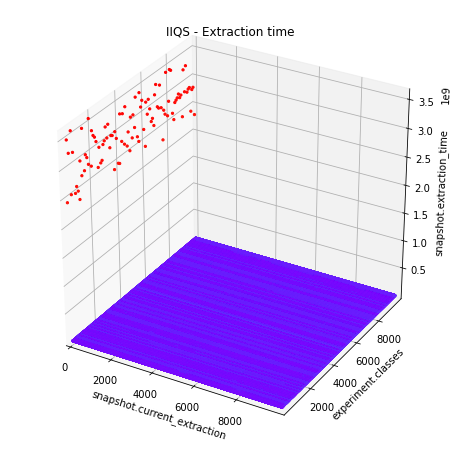
\includegraphics[height=0.6\textheight]{chapter4/01-basebenchmark-05-classes.png.0-1.png}
            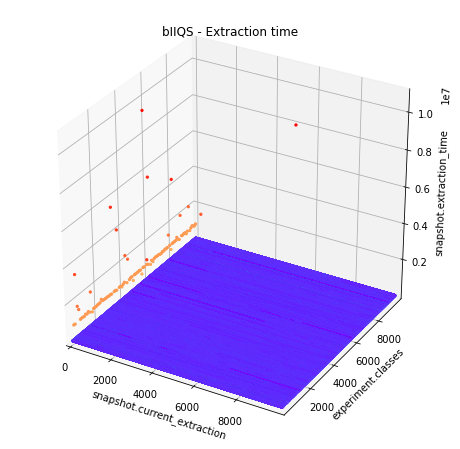
\includegraphics[height=0.6\textheight]{chapter5/01-basebenchmark-05-classes.png.0-1.png}
        \end{subfigure}
        \caption{Impact of classes on BIIQS execution.}
    \end{figure}
    \note[item]{adicionalmente, podemos ver una baja importante en el orden de magnitud de la primera extracción del mismo sobre la cual la cantidad de clases no afecta su tiempo de ejecucuón de ninguna forma.}
\end{frame}



\begin{frame}{Bias impact}
    \begin{figure}
        \centering
        \begin{subfigure}[b]{\textwidth}
            \centering
            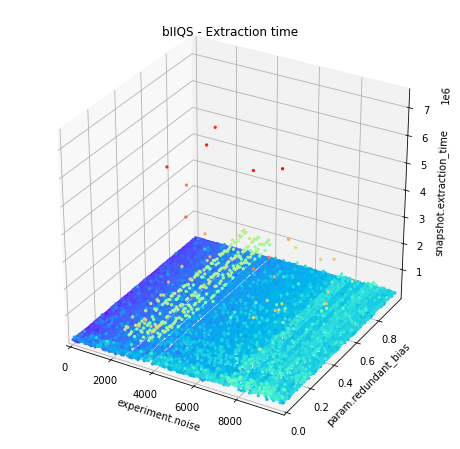
\includegraphics[height=0.6\textheight]{chapter5/01-basebenchmark-06-noise-redundant-bias.png.0-0.png}
            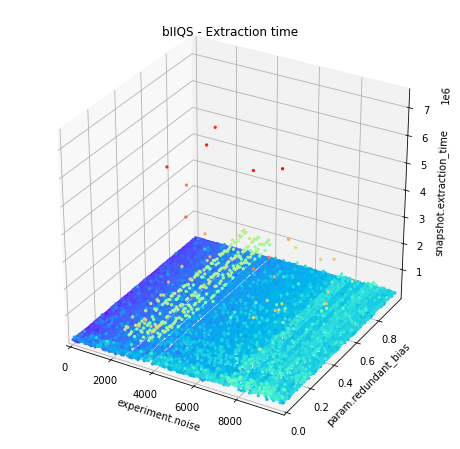
\includegraphics[height=0.6\textheight]{chapter5/01-basebenchmark-06-noise-redundant-bias.png.0-0.png}
        \end{subfigure}
        \caption{Impact of random noise and partition bias on IIQS execution.}
    \end{figure}
    \note[item]{Una gran diferencia por sobre la implementación original, es que ahora ni el sesgo de partición ni el ruido aleatorio cambian el tiempo de ejecución. }
    \note[item]{Incluso para las combinaciones donde el fallo de cache es constante, se mantiene dentro de los márgenes aceptables de ejecución.}
    \note[item]{De hecho, ni siquiera fue necesario utilizar una escala logaritmica.}
\end{frame}




\section{Summary}

\begin{frame}{summary}
    \begin{itemize}
        \item We have presented bIIQS, an alternative to IIQS which provides support for repeated elements on its input sequence, in optimal time and space.
        \item We have provided with a starter framework to replicate the process by using an experimental algorithmics approach.
        \item We delivered an experimental analysis of those three algorithms along with a portable implementation.
    \end{itemize}
\end{frame}

\subsection{Future work}

\begin{frame}{summary}
    \begin{itemize}
        \item Constrain timing test by using specialized hardware implementations.
        \item Develop a full theoretical analysis of both IIQS and bIIQS.
    \end{itemize}
\end{frame}


\begin{frame}
    \titlepage
  \end{frame}

\end{document}
